\documentclass[border=4pt]{standalone}

\usepackage{tikz} 
\usetikzlibrary{shapes,arrows,positioning,automata,backgrounds,calc,er,patterns}
\usepackage{tikz-feynman}
\tikzfeynmanset{compat=1.0.0}
 \usepackage{physics}
 
  %Use LuaLaTex to compile
\begin{document}
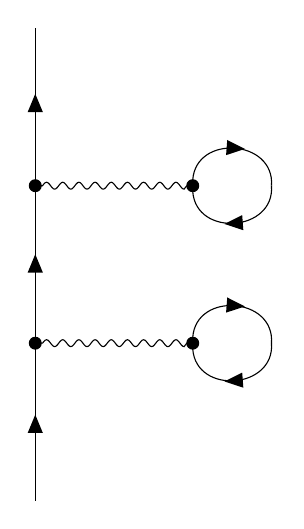
\begin{tikzpicture}
  \begin{feynman}
    %vertical
    \vertex (x) at (0,6);
    \vertex [dot] (x2) at (0, 4) {};
    \vertex [dot] (x1) at (0, 2) {};
    \vertex (y) at (0, 0);
    %horizontal
    \vertex [dot] (x2p) at (2,4) {};
    \vertex [dot] (x1p) at (2,2) {};
    %loop
    \vertex (x2pp) at (3,4);
    \vertex (x1pp) at (3,2);        
    \diagram*
        { 
          (y)  -- [fermion] (x1) -- [photon] (x1p) -- [fermion, half left] (x1pp) -- [fermion, half left] (x1p),          
          (x1) -- [fermion] (x2) -- [photon] (x2p) -- [fermion, half left] (x2pp) -- [fermion, half left] (x2p),
          (x2) -- [fermion] (x),
        };
  \end{feynman}
\end{tikzpicture}

\end{document}
%{\(x\) {\scriptsize \( \alpha \)}}